\documentclass[11pt,twoside]{book}

% Reutiliza la misma plantilla y paleta del Volumen I, para que la
% colección se lea como una sola obra (ver CLAUDE.md y ROADMAP.md).
% ============================================================
% estilo.tex — Plantilla visual del libro guía
% Teoría Matemática de la Luz (H. Poincaré) — edición en español
% ============================================================

% ---------- Geometría de página: más texto por página ----------
\usepackage[
  paperwidth=17cm,paperheight=24cm,
  inner=2cm,outer=1.8cm,top=2.2cm,bottom=2.4cm,
  headheight=36pt,includeheadfoot
]{geometry}

% ---------- Tipografía y codificación ----------
\usepackage[spanish,es-noindentfirst]{babel}
\usepackage[utf8]{inputenc}
\usepackage[T1]{fontenc}
\usepackage{newpxtext,newpxmath} % serif de corte clásico, afín al original de 1889
\usepackage{microtype}

% ---------- Matemáticas ----------
% newpxmath ya redefine \Bbbk y \openbox; se evita el choque con
% amssymb/amsthm (no se usan entornos de teorema: se usan las cajas
% tcolorbox definidas más abajo).
\usepackage{amsmath}
\let\Bbbk\relax
\usepackage{amssymb}
\usepackage{mathtools}

% ---------- Color: paleta del libro ----------
\usepackage{xcolor}
\definecolor{azulpoincare}{HTML}{14315D}      % azul profundo — títulos, estructura
\definecolor{azulclaro}{HTML}{E8EEF5}         % azul muy claro — fondo de cajas de definición
\definecolor{rojopoincare}{HTML}{9E1B32}      % rojo — acentos, cálculos, numeración
\definecolor{rojoclaro}{HTML}{F7E9EA}         % rojo muy claro — fondo de cajas de cálculo
\definecolor{grisnota}{HTML}{4A4A4A}          % gris — notas históricas

% ---------- Figuras y cajas ----------
\usepackage{graphicx}
\usepackage[most]{tcolorbox}
\tcbuselibrary{skins,breakable}

% ---------- Encabezados ----------
\usepackage{fancyhdr}
\usepackage{titlesec}
\usepackage{enumitem}
\usepackage{hyperref}
\hypersetup{
  colorlinks=true,
  linkcolor=azulpoincare,
  citecolor=rojopoincare,
  urlcolor=azulpoincare,
  % Poincaré reinicia su numeración de ecuaciones muchas veces por
  % capítulo; sin esto, hyperref genera anclas duplicadas (equation.N.M).
  hypertexnames=false,
  pdftitle={Teoría Matemática de la Luz — Henri Poincaré},
}

% ============================================================
% Portadilla de capítulo — imita la composición tipográfica
% original ("CHAPITRE N" / título centrado, filete, blanco)
% pero en español y con la paleta azul/rojo
% ============================================================
% El cuerpo del texto cita los capítulos en números romanos ("Capítulo
% III", como en el original francés "CHAPITRE III"); la portadilla debe
% coincidir con esa misma convención.
\renewcommand{\thechapter}{\Roman{chapter}}

\titleformat{\chapter}[display]
  {\normalfont\centering}
  {\color{rojopoincare}\Large\scshape Capítulo \thechapter}
  {12pt}
  {\color{azulpoincare}\Huge\bfseries\scshape}
\titlespacing*{\chapter}{0pt}{80pt}{40pt}

\renewcommand{\thesection}{\thechapter.\arabic{section}}

% Los números de capítulo en romanos ("VIII.8.8") son más anchos que en
% arábigos; se ensancha la columna de numeración del índice general para
% que quepan sin desbordar.
\makeatletter
\renewcommand{\l@section}{\@dottedtocline{1}{1.5em}{3.3em}}
\renewcommand{\l@subsection}{\@dottedtocline{2}{4.0em}{4.2em}}
% Índice de figuras: "VIII.6." es más ancho que "6.".
\renewcommand{\l@figure}{\@dottedtocline{1}{1em}{3.5em}}
% Índice general, entradas de capítulo: ensanchar la sangría de
% continuación para que quepa "VIII. " cuando el título se parte en
% más de una línea.
\renewcommand{\l@chapter}[2]{%
  \ifnum \c@tocdepth >\m@ne
    \addpenalty{-\@highpenalty}%
    \vskip 1.0em \@plus\p@
    \setlength\@tempdima{2.8em}%
    \begingroup
      \parindent \z@ \rightskip \@pnumwidth
      \parfillskip -\@pnumwidth
      \leavevmode \bfseries
      \advance\leftskip\@tempdima
      \hskip -\leftskip
      #1\nobreak\hfil
      \nobreak\hb@xt@\@pnumwidth{\hss #2}\par
      \penalty\@highpenalty
    \endgroup
  \fi}
\makeatother

% Numeración de ecuaciones: se muestra solo el número de Poincaré, "(5)",
% sin prefijo de capítulo, tanto si se fija con \tag{N} como si se deja
% al contador automático (con \setcounter{equation}{..} en cada reinicio
% del original). Así todos los capítulos muestran el mismo formato.
\renewcommand{\theequation}{\arabic{equation}}

% ============================================================
% Cajas de estilo "libro guía"
% ============================================================

% Nota sobre los cálculos que extendemos: NO llevan caja, ni encabezado,
% ni pasos numerados, ni subtítulos en negrilla. Se escriben como
% continuación en prosa del propio texto, en el mismo registro que
% Poincaré, como una simple ampliación de lo que él deja implícito — no
% como un aparato pedagógico aparte. Ver CLAUDE.md.

% --- Enunciado importante / principio / resultado clave ---
% Para destacar afirmaciones centrales (principios, resultados
% culminantes), NO para sus demostraciones.
\newtcolorbox{enunciado}[1]{%
  breakable,
  enhanced,
  colback=azulclaro,
  colframe=azulpoincare,
  boxrule=0.6pt,
  left=8pt,right=8pt,top=6pt,bottom=6pt,
  fonttitle=\bfseries\color{white},
  coltitle=white,
  colbacktitle=azulpoincare,
  title={#1},
  attach boxed title to top left={xshift=8pt,yshift=-2mm},
  boxed title style={colback=azulpoincare,boxrule=0pt,sharp corners},
}

% --- Nota histórica / contexto ---
\newtcolorbox{notahistorica}[1][]{%
  breakable,
  enhanced,
  colback=white,
  colframe=grisnota,
  boxrule=0.5pt,
  left=8pt,right=8pt,top=6pt,bottom=6pt,
  fonttitle=\itshape\color{grisnota},
  coltitle=grisnota,
  title={Nota histórica#1},
  attach boxed title to top left={xshift=8pt,yshift=-2mm},
  boxed title style={colback=white,colframe=grisnota,boxrule=0.5pt,sharp corners},
}

% --- Definición / concepto clave ---
\newtcolorbox{definicion}[1][]{%
  breakable,
  enhanced,
  colback=azulclaro,
  colframe=azulpoincare,
  boxrule=0.6pt,
  left=8pt,right=8pt,top=6pt,bottom=6pt,
  fonttitle=\bfseries\color{white},
  coltitle=white,
  colbacktitle=azulpoincare,
  title={Definición#1},
  attach boxed title to top left={xshift=8pt,yshift=-2mm},
  boxed title style={colback=azulpoincare,boxrule=0pt,sharp corners},
}

% ============================================================
% Ecuaciones: numeración doble (libro guía + referencia original)
% Uso: \begin{ecnum}{III.4}{orig. (4)} ... \end{ecnum}
% ============================================================
\newenvironment{ecnum}[2]{%
  \gdef\ecnumA{#1}\gdef\ecnumB{#2}%
  \begin{equation}%
}{%
  \tag{\ecnumA\ \text{\footnotesize[\ecnumB]}}%
  \end{equation}%
}

% ---------- Pie de página no justificado verticalmente ----------
% Con \flushbottom (predeterminado en twoside), las páginas que preceden a
% una nota al pie larga, una figura o una caja no divisible se estiran y
% dejan huecos grandes entre ecuaciones (avisos "Underfull \vbox"). Con
% \raggedbottom el texto conserva su espaciado natural y el sobrante queda
% al pie de la página. Para volver al comportamiento anterior, borrar esta
% línea.
\raggedbottom

% ---------- Encabezado de página (estilo "guía de lectura") ----------
\setlength{\headheight}{36pt}
\pagestyle{fancy}
\fancyhf{}
\fancyhead[LE,RO]{\thepage}
\fancyhead[RE]{\color{azulpoincare}\scshape\nouppercase{\leftmark}}
\fancyhead[LO]{\color{azulpoincare}\scshape\nouppercase{\rightmark}}
\renewcommand{\headrulewidth}{0.4pt}
\renewcommand{\headrule}{\hbox to\headwidth{\color{rojopoincare}\leaders\hrule height \headrulewidth\hfill}}


\title{Teoría Matemática de la Luz II}
\author{Henri Poincaré}
\date{}

\begin{document}

% ============================================================
% portada.tex — Portadilla textual del volumen
% Imita la composición tipográfica de la portada original de 1892
% (no la pasta física del libro), en español y paleta azul/rojo.
% Mismo estilo que volumen-1/00-frontmateria/portada.tex.
% ============================================================
\begin{titlepage}
\centering
\vspace*{1.5cm}

{\color{azulpoincare}\small\scshape Curso de la Facultad de Ciencias de París\par}
{\color{grisnota}\footnotesize publicado por la asociación amical de alumnos y exalumnos\par
de la Facultad de Ciencias\par}

\vspace{2pt}
\color{rojopoincare}\rule{0.55\textwidth}{0.6pt}
\color{black}
\vspace{18pt}

{\color{azulpoincare}\scshape\large Curso de Física Matemática\par}

\vspace{28pt}

{\color{azulpoincare}\scshape\Large Teoría Matemática\par}
{\color{azulpoincare}\scshape\large de\par}
{\color{azulpoincare}\bfseries\scshape\Huge La Luz\par}

\vspace{10pt}
{\color{rojopoincare}\large II\par}

\vspace{20pt}

{\small Volumen II — Edición guía en español latino\par}
{\footnotesize Nuevos estudios sobre la difracción. Teoría de la\par
dispersión de Helmholtz\par}
{\footnotesize Traducción, desarrollo explícito de cálculos y figuras vectoriales\par
a partir de las lecciones profesadas por H.\,Poincaré durante\par
el primer semestre de 1891-1892\par}

\vspace{40pt}

{\scshape por\par}
\vspace{4pt}
{\Large\bfseries H.\ Poincaré}, {\small miembro del Instituto\par}

\vspace{6pt}
{\footnotesize redactadas originalmente por M.\ Lamotte y D.\ Hurmuzescu,\par
licenciados en ciencias\par}

\vfill

\color{rojopoincare}\rule{0.35\textwidth}{0.6pt}\color{black}

\vspace{14pt}
{\footnotesize Edición y traducción al español latino, \the\year\par}

\end{titlepage}


% Pendiente: prólogo del traductor para este volumen (breve, remite al
% prólogo del Volumen I) e Introducción original de Poincaré traducida.
% \input{00-frontmateria/introduccion}

\tableofcontents

\listoffigures

% Capítulos — se añaden a medida que se traducen:
% % ============================================================
% Capítulo I (Volumen II) — Teoría elástica de la luz
% Traducción de "Théorie mathématique de la lumière II" (1892)
% Original: §§1-11, páginas impresas 1-18
% ============================================================
\chapter{Teoría elástica de la luz}
\label{cap:vol2-elastica}

\section{Movimiento del éter}

\noindent\textbf{1. Movimiento del éter.} — Esta teoría atribuye los
fenómenos luminosos a las vibraciones de un medio elástico, el éter,
difundido en todo el espacio, incluso en el vacío.

Sea una molécula de éter que, en el estado de equilibrio, ocupa la
posición $M$: a consecuencia de la vibración, vendrá a ocupar una posición
tal como $M'$. El vector $MM'$ se llama el desplazamiento de la molécula.
Si $x,y,z$ designan las coordenadas del punto $M$, y $x+\xi,\,y+\eta,\,z+\zeta$
las del punto $M'$, las proyecciones del desplazamiento sobre los tres ejes
de coordenadas serán $\xi,\eta,\zeta$.

Las componentes de la velocidad de la molécula según los mismos ejes serán
\[
\frac{d\xi}{dt},\qquad \frac{d\eta}{dt},\qquad \frac{d\zeta}{dt},
\]
y las componentes de la aceleración
\[
\frac{d^2\xi}{dt^2},\qquad \frac{d^2\eta}{dt^2},\qquad \frac{d^2\zeta}{dt^2}.
\]

Consideremos un pequeño paralelepípedo rectángulo $ABCDEFGH$
(figura~\ref{fig:vol2-cap1-1}), cuyas aristas sean paralelas a los ejes y tengan
respectivamente por longitud $dx,dy,dz$: el volumen de este paralelepípedo
será $d\tau=dx\,dy\,dz$. Durante la vibración, este paralelepípedo se
desplaza y toma una posición tal como $A'B'C'D'E'F'G'H'$; se convierte en
un paralelepípedo curvilíneo, que puede asimilarse, despreciando
infinitésimos de segundo orden, a un paralelepípedo rectilíneo, pero
oblicuo.

Pongamos
\[
\alpha_1=\frac{d\xi}{dx},\qquad \alpha_2=\frac{d\eta}{dy},\qquad \alpha_3=\frac{d\zeta}{dz};
\]
\[
\beta_1=\frac{d\eta}{dz}+\frac{d\zeta}{dy};\qquad
\beta_2=\frac{d\zeta}{dx}+\frac{d\xi}{dz};\qquad
\beta_3=\frac{d\xi}{dy}+\frac{d\eta}{dx}.
\]
Se demuestra (véase el \emph{Cours d'élasticité}, p.~7) que las longitudes
de las aristas del paralelepípedo se convierten en
\[
dx(1+\alpha_1)\qquad dy(1+\alpha_2)\qquad dz(1+\alpha_3).
\]
Por esta razón $\alpha_1,\alpha_2,\alpha_3$ se llaman las dilataciones
lineales.

Los tres ángulos del triedro $A$, que eran los tres iguales a $\pi/2$, se
convierten respectivamente, en el triedro $A'$, en
\[
\frac{\pi}{2}+\beta_1,\qquad \frac{\pi}{2}+\beta_2,\qquad \frac{\pi}{2}+\beta_3.
\]
$\beta_1,\beta_2,\beta_3$ se llaman las dilataciones angulares.

En cuanto a la diagonal $AH$, se convierte en $A'H'$, y su longitud es
función de las seis dilataciones.

\begin{figure}[ht]
\centering
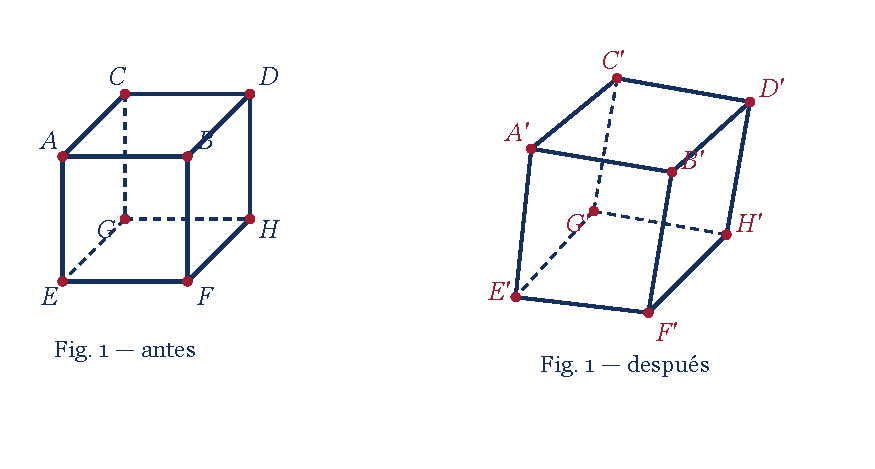
\includegraphics[width=0.85\textwidth]{figuras/pdf/cap01-fig1.pdf}
\caption{El paralelepípedo $ABCDEFGH$ antes y después de la vibración,
convertido en el paralelepípedo oblicuo $A'B'C'D'E'F'G'H'$.}
\label{fig:vol2-cap1-1}
\end{figure}

\section{Fuerza viva del éter}

\noindent\textbf{2. Fuerza viva del éter.} — Sea $\mathrm{T}$ la fuerza
viva o energía cinética del éter.\footnote{A diferencia del Volumen~I,
donde «fuerza viva» designa $\sum mv^2$, el doble de la energía cinética,
aquí Poincaré identifica expresamente la fuerza viva con la energía
cinética $\sum mv^2/2$, como muestra la expresión de $\mathrm{T}$ que
sigue. Conservamos el término tal como él lo usa.~(N.~del T.)} Tenemos, como expresión del cuadrado de
la velocidad,
\[
V^2=\left(\frac{d\xi}{dt}\right)^2+\left(\frac{d\eta}{dt}\right)^2+\left(\frac{d\zeta}{dt}\right)^2.
\]
La masa del pequeño paralelepípedo es $\rho\,d\tau$, siendo $\rho$ la
densidad del éter. Por consiguiente
\[
\mathrm{T}=\sum\frac{mv^2}{2}
=\frac{1}{2}\int\rho\,d\tau\left[\left(\frac{d\xi}{dt}\right)^2
+\left(\frac{d\eta}{dt}\right)^2+\left(\frac{d\zeta}{dt}\right)^2\right].
\]

\section{Energía potencial del éter}

\noindent\textbf{3. Energía potencial del éter.} — Se ha demostrado, en el
\emph{Cours d'élasticité}, p.~43, §26 y siguientes, que la energía
potencial tenía una expresión de la forma
\[
\mathrm{U}=\int \mathrm{W}\,d\tau,
\]
siendo $\mathrm{W}$ un polinomio de segundo grado respecto de las nueve
derivadas parciales de primer orden de $\xi,\eta,\zeta$.

Si suponemos que el medio es isótropo y que en el estado de equilibrio la
presión es nula, obtendremos
\[
\mathrm{W}=\mu\left(\alpha_1^2+\alpha_2^2+\alpha_3^2
+\frac{\beta_1^2}{2}+\frac{\beta_2^2}{2}+\frac{\beta_3^2}{2}\right)+\lambda\frac{\theta^2}{2}.
\]
$\lambda$ y $\mu$ son los coeficientes de Lamé; $\theta$ está definido por
la igualdad
\[
\theta=\alpha_1+\alpha_2+\alpha_3=\frac{d\xi}{dx}+\frac{d\eta}{dy}+\frac{d\zeta}{dz}.
\]
Se demuestra que un elemento de volumen $d\tau$ se convierte, tras la
deformación, en
\[
d\tau(1+\theta),
\]
de donde el nombre de dilatación cúbica dado a $\theta$.

\section{Valor de las fuerzas}

\noindent\textbf{4. Valor de las fuerzas.} — Retomemos el paralelepípedo
$ABCDEFGH$, y consideremos en particular la cara $ACEG$ perpendicular a
$Ox$ (figura~\ref{fig:vol2-cap1-2}): el área de esta cara es igual a
$dy\,dz$. Llamaremos $\mathrm{P}_{xx},\mathrm{P}_{xy},\mathrm{P}_{xz}$ a
las componentes según los ejes de la presión que se ejerce sobre esta cara
por unidad de área, y convendremos en considerar las tensiones como
positivas, y las presiones como negativas.

Las componentes de la presión que se ejerce sobre la cara $ACEG$ serán,
pues,
\[
\mathrm{P}_{xx}\,dy\,dz,\qquad \mathrm{P}_{xy}\,dy\,dz,\qquad \mathrm{P}_{xz}\,dy\,dz.
\]
Tendremos del mismo modo, para la cara $ABEF$ perpendicular a $Oy$,
\[
\mathrm{P}_{yx}\,dx\,dz,\qquad \mathrm{P}_{yy}\,dx\,dz,\qquad \mathrm{P}_{yz}\,dx\,dz,
\]
y para la cara $EFGH$ perpendicular a $Oz$,
\[
\mathrm{P}_{zx}\,dx\,dy,\qquad \mathrm{P}_{zy}\,dx\,dy,\qquad \mathrm{P}_{zz}\,dx\,dy.
\]
Según la teoría de la elasticidad,
\[
\mathrm{P}_{xy}=\mathrm{P}_{yx}\qquad \mathrm{P}_{yz}=\mathrm{P}_{zy}\qquad \mathrm{P}_{zx}=\mathrm{P}_{xz}
\]
y
\[
\mathrm{P}_{xx}=\frac{d\mathrm{W}}{d\alpha_1}=\lambda\theta\frac{d\theta}{d\alpha_1}+2\mu\alpha_1
=\lambda\theta+2\mu\alpha_1=\lambda\theta+2\mu\frac{d\xi}{dx}
\]
\[
\mathrm{P}_{yy}=\lambda\theta+2\mu\frac{d\eta}{dy}
\]
\[
\mathrm{P}_{zz}=\lambda\theta+2\mu\frac{d\zeta}{dz}
\]
\[
\mathrm{P}_{xy}=\mu\beta_3=\mu\left(\frac{d\xi}{dy}+\frac{d\eta}{dx}\right)
\]

\begin{figure}[ht]
\centering
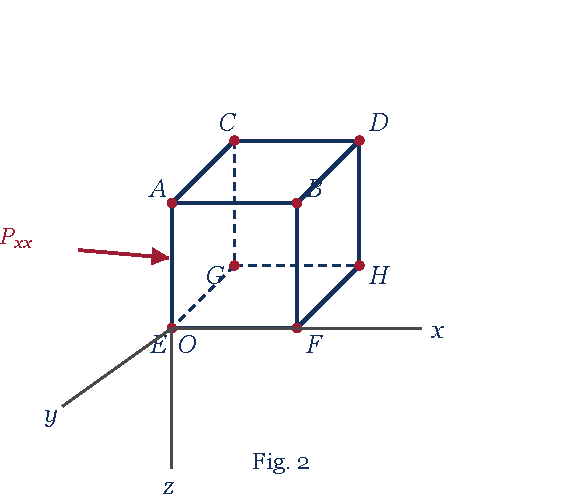
\includegraphics[width=0.7\textwidth]{figuras/pdf/cap01-fig2.pdf}
\caption{La cara $ACEG$, perpendicular a $Ox$, sobre la que se ejerce la
presión $\mathrm{P}_{xx}$.}
\label{fig:vol2-cap1-2}
\end{figure}

\section{Ecuaciones del movimiento}

\noindent\textbf{5. Ecuaciones del movimiento.} — Escribiendo que la
fuerza de inercia equilibra a las fuerzas que actúan sobre el elemento
$d\tau$, obtendremos las ecuaciones del movimiento:\footnote{En la
expresión que sigue, el original imprime $dy\,dx$ como último factor del
segundo renglón y $d\mathrm{P}_{xz}/dx$ en el tercero, y escribe
$d^2\zeta/dt^2$ en el primer miembro de la ecuación~(1); son
erratas evidentes por $dz\,dx$ (área de la cara perpendicular a $Oy$),
$d\mathrm{P}_{xz}/dz$ y $d^2\xi/dt^2$, como muestran el
primer miembro de la expresión desarrollada y la ecuación que se obtiene a
continuación por sustitución.~(N.~del T.)}
\[
\begin{aligned}
\rho\,dx\,dy\,dz\cdot\frac{d^2\xi}{dt^2}
={}&-\mathrm{P}_{xx}\,dy\,dz+\left(\mathrm{P}_{xx}+\frac{d\mathrm{P}_{xx}}{dx}dx\right)dy\,dz\\
&-\mathrm{P}_{xy}\,dz\,dx+\left(\mathrm{P}_{xy}+\frac{d\mathrm{P}_{xy}}{dy}dy\right)dz\,dx\\
&-\mathrm{P}_{xz}\,dx\,dy+\left(\mathrm{P}_{xz}+\frac{d\mathrm{P}_{xz}}{dz}dz\right)dx\,dy
\end{aligned}
\]
o bien
\begin{equation}
\rho\frac{d^2\xi}{dt^2}=\frac{d\mathrm{P}_{xx}}{dx}+\frac{d\mathrm{P}_{xy}}{dy}+\frac{d\mathrm{P}_{xz}}{dz}
\tag{1}
\end{equation}
y otras dos que se obtendrían por permutación. Por otra parte,
\[
\mathrm{P}_{xx}=\mu\frac{d\xi}{dx}+\mu\frac{d\xi}{dx}+\lambda\theta,\qquad
\mathrm{P}_{xy}=\mu\frac{d\xi}{dy}+\mu\frac{d\eta}{dx},\qquad
\mathrm{P}_{xz}=\mu\frac{d\xi}{dz}+\mu\frac{d\zeta}{dx}.
\]
Sustituyendo estas expresiones en la ecuación (1), resulta
\[
\rho\frac{d^2\xi}{dt^2}=\mu\Delta\xi+\mu\frac{d\theta}{dx}+\lambda\frac{d\theta}{dx}.
\]
Las ecuaciones del movimiento serán, pues,
\begin{equation}
\begin{gathered}
\rho\frac{d^2\xi}{dt^2}=\mu\Delta\xi+(\lambda+\mu)\frac{d\theta}{dx},\\[3pt]
\rho\frac{d^2\eta}{dt^2}=\mu\Delta\eta+(\lambda+\mu)\frac{d\theta}{dy},\\[3pt]
\rho\frac{d^2\zeta}{dt^2}=\mu\Delta\zeta+(\lambda+\mu)\frac{d\theta}{dz}.
\end{gathered}
\tag{I}
\end{equation}

\section{Ondas planas}
\label{sec:vol2-cap1-ondas-planas-1}

\noindent\textbf{6. Ondas planas.} — En el caso de las ondas planas,
$\xi$ y $\eta$ no dependen más que de $z$ y de $t$. Por consiguiente,
\[
\Delta\xi=\frac{d^2\xi}{dz^2}\qquad \Delta\eta=\frac{d^2\eta}{dz^2}\qquad
\theta=\frac{d\zeta}{dz}\qquad \Delta\zeta=\frac{d^2\zeta}{dz^2}.
\]
Las derivadas tomadas respecto de $x$ y de $y$ son nulas, y las ecuaciones
del movimiento se reducen a
\[
\rho\frac{d^2\xi}{dt^2}=\mu\frac{d^2\xi}{dz^2}\qquad
\rho\frac{d^2\eta}{dt^2}=\mu\frac{d^2\eta}{dz^2}\qquad
\rho\frac{d^2\zeta}{dt^2}=\mu\frac{d^2\zeta}{dz^2}+(\lambda+\mu)\frac{d^2\zeta}{dz^2}
=(\lambda+2\mu)\frac{d^2\zeta}{dz^2}.
\]
Estas ecuaciones son las de las cuerdas vibrantes.

Supongamos que el desplazamiento sea paralelo a $Ox$:
\[
\eta=\zeta=0 \qquad \xi\neq 0.
\]
El plano de onda es paralelo al plano $xy$. La vibración es transversal.
Solo queda, pues, la ecuación
\[
\rho\frac{d^2\xi}{dt^2}=\mu\frac{d^2\xi}{dz^2}.
\]
Esta ecuación tiene por integral
\[
\xi=f\left(z+t\sqrt{\frac{\mu}{\rho}}\right)+f_1\left(z-t\sqrt{\frac{\mu}{\rho}}\right),
\]
siendo $f$ y $f_1$ funciones arbitrarias. Esta onda se propaga con la
velocidad $\sqrt{\mu/\rho}$.

Habríamos obtenido un resultado enteramente análogo suponiendo el
desplazamiento paralelo a $Oy$.

Si el desplazamiento es paralelo a $Oz$, subsiste únicamente la ecuación
\[
\rho\frac{d^2\zeta}{dt^2}=(\lambda+2\mu)\frac{d^2\zeta}{dz^2}.
\]
La integral
\[
\zeta=f\left(z+t\sqrt{\frac{\lambda+2\mu}{\rho}}\right)+f_1\left(z-t\sqrt{\frac{\lambda+2\mu}{\rho}}\right)
\]
representa una vibración longitudinal, puesto que el desplazamiento es
perpendicular al plano de onda, y la velocidad de propagación es
$\sqrt{(\lambda+2\mu)/\rho}$.

La experiencia nos enseña que las vibraciones luminosas son transversales.
En efecto, en los diversos fenómenos de reflexión o de refracción, se
recupera toda la fuerza viva del rayo incidente en los rayos de vibraciones
transversales. Si existieran rayos de vibraciones longitudinales, estos
absorberían una parte de esta fuerza viva.

Admitiremos, pues, que no existe vibración longitudinal en el rayo
luminoso, y por consiguiente que
\[
\lambda+2\mu=0.
\]

\section{Intensidad luminosa. Definición experimental}

\noindent\textbf{7. Intensidad luminosa. Definición experimental.} — Para
poder comparar con la experiencia las consecuencias de las ecuaciones, es
indispensable definir bien la cantidad que se mide en las experiencias, es
decir, la intensidad luminosa.

Es necesario incluso dar de esta intensidad dos definiciones, una
experimental, y la otra teórica; pues queremos comparar la teoría con la
experiencia, y para que esta comparación sea posible, hay que definir bien
los dos términos.

Experimentalmente, la intensidad se mide con ayuda de tres clases de
fenómenos: $1.^{\text{o}}$ los efectos fisiológicos; $2.^{\text{o}}$ los
efectos químicos (fotográficos); $3.^{\text{o}}$ los efectos caloríficos de
la luz. A cada una de estas clases de fenómenos corresponde una definición
de la intensidad. No es evidente \emph{a priori} que estas tres
definiciones sean equivalentes, y de hecho no lo son en absoluto. Sabemos,
por ejemplo, que la intensidad de la acción química de un rayo varía con su
color. Cuando se trata de comparar dos rayos homogéneos del mismo color, es
posible que el efecto fisiológico sea proporcional al efecto químico, y
así parece ocurrir en el caso de una onda plana; pero en los casos más
delicados, como en las experiencias recientes del señor Otto Wiener, solo
es posible un modo de evaluación, el que está fundado en la fotografía.

Somos, sin embargo, libres de adoptar una de estas definiciones y de
examinar sus consecuencias.

Convendremos, pues, en decir que dos luces tienen igual intensidad cuando
producen en el mismo tiempo la misma acción sobre una placa fotográfica;
que una luz tiene una intensidad mayor o menor que otra según que, en el
mismo tiempo, produzca sobre la placa sensible una acción mayor o menor
que esa otra.

Esta definición es puramente experimental.

\section{Definición teórica}

\noindent\textbf{8. Definición teórica.} — Desde el punto de vista
teórico, se ha considerado a menudo la intensidad como proporcional a la
fuerza viva media o energía cinética del éter.

Esta fuerza viva del éter, para el elemento de volumen $d\tau$, es igual a
\[
\rho\,d\tau\cdot\frac{v^2}{2},
\]
es decir, por unidad de masa, $v^2/2$.

Supongamos, por ejemplo, que la vibración sea rectilínea y tomemos como
eje de las $x$ la dirección de vibración en el punto considerado; entonces
\[
\eta=\zeta=0 \qquad v=\frac{d\xi}{dt};
\]
la fuerza viva será
\[
\frac{1}{2}\left(\frac{d\xi}{dt}\right)^2,
\]
y la intensidad será proporcional al valor medio de esta expresión.

Siendo el movimiento periódico, podemos poner
\[
\xi=\mathrm{A}\sin 2\pi\frac{t}{\mathrm{T}},
\]
eligiendo como origen del tiempo el instante en que $\xi=0$; $\mathrm{T}$
es el período; $\xi$ tiene por máximo $\mathrm{A}$ en valor absoluto;
$\mathrm{A}$ es la amplitud.
\[
\frac{d\xi}{dt}=\mathrm{A}\frac{2\pi}{\mathrm{T}}\cos 2\pi\frac{t}{\mathrm{T}}.
\]
La intensidad será, pues, proporcional a\footnote{El original da como
valor de esta integral $(\mathrm{A}^2/2)(4\pi^2/\mathrm{T}^2)$,
olvidando el factor $\frac12$ que proviene del valor medio de
$\cos^2 2\pi t/\mathrm{T}$ sobre un período. La omisión no afecta la
conclusión, que solo concierne a la proporcionalidad con
$\mathrm{A}^2$.~(N.~del T.)}
\[
\frac{1}{\mathrm{T}}\int_0^{\mathrm{T}}\frac{\mathrm{A}^2}{2}\frac{4\pi^2}{\mathrm{T}^2}
\cos^2 2\pi\frac{t}{\mathrm{T}}\,dt=\frac{1}{2}\cdot\frac{\mathrm{A}^2}{2}\frac{4\pi^2}{\mathrm{T}^2}.
\]
Es, pues, proporcional al cuadrado de la amplitud $\mathrm{A}$.

No es en absoluto evidente que así definamos la misma cosa que con la
definición experimental. Estamos tan autorizados a suponer que la acción
fotográfica es proporcional, no a la energía cinética media, sino a la
energía potencial o a la energía total media.

\noindent\textbf{9.} Estas diversas definiciones de la intensidad,
equivalentes en ciertos casos, como vamos a verlo, corresponden a maneras
distintas de concebir el mecanismo de la acción fotográfica.

Consideremos, en efecto, las moléculas de éter que, en su posición de
equilibrio, ocupan una esfera infinitamente pequeña $O$. Cuando el éter
entre en vibración, el centro de gravedad de la esfera oscilará de un lado
y otro de $O$, y al mismo tiempo la esfera se deformará: tomará una forma
asimilable a la de un elipsoide $O'$ (figura~\ref{fig:vol2-cap1-3}); los
ejes de este elipsoide ejecutarán también una serie de oscilaciones.

¿Depende la intensidad de la amplitud de las oscilaciones de $O$, o está
relacionada con la amplitud de las oscilaciones de los ejes del elipsoide?
No lo sabemos.

Si admitimos que la intensidad es proporcional a la fuerza viva media,
como las componentes de la velocidad son $d\xi/dt,d\eta/dt,d\zeta/dt$, la
intensidad dependerá de la variación de $\xi,\eta,\zeta$ con el tiempo, es
decir, del desplazamiento del punto $O$. Admitamos, al contrario, que la
intensidad es proporcional a la energía potencial media $\int \mathrm{W}\,d\tau$;
$\mathrm{W}$ depende de las dilataciones $\alpha$ y $\beta$; o bien aún de
los ejes del elipsoide (cf. \emph{Théorie de l'Élasticité}, p.~9); la
intensidad dependería entonces de la amplitud de las deformaciones de la
esfera, es decir, de las variaciones periódicas que experimenta la
distancia de dos moléculas, variaciones que son función de las $\alpha$ y
de las $\beta$.

Ignoramos la naturaleza de las acciones químicas de las que son sede las
placas fotográficas. Sin duda los átomos materiales correspondientes
experimentan el mismo desplazamiento, y podría uno sentirse tentado a
razonar así:

Supongamos que el desplazamiento del punto $O$ sea considerable, y las
deformaciones del elipsoide muy pequeñas. Nuestra esfera estará sometida
únicamente a un movimiento de traslación; la distancia de dos moléculas de
éter permanecerá invariable durante la vibración, y lo mismo ocurrirá con
la distancia de dos átomos materiales, puesto que hemos supuesto que el
desplazamiento del éter es el mismo que el de la materia ponderable. En
esta hipótesis se comprende difícilmente la disociación de la molécula
química. No podría, pues, haber acción química, por grande que fuera el
desplazamiento del punto $O$, cuando el elipsoide no se deformara. Se
concluiría, pues, que la intensidad depende de las variaciones de las
$\alpha$ y de las $\beta$, y no de las de $\xi,\eta,\zeta$.

Pero esta manera de ver no se impone.

Nada impide suponer que el desplazamiento del éter y el del átomo material
sean solo proporcionales, variando el coeficiente de proporcionalidad de un
átomo a otro, y se llegaría a una conclusión inversa.

En el primer orden de ideas, la intensidad sería proporcional a la energía
potencial media; en el segundo caso, a la fuerza viva media.

Pero, repitámoslo, ninguna de estas hipótesis se impone necesariamente.

Por lo demás, en la mayoría de los casos, y son justamente los únicos que,
hasta estos últimos años, hemos conseguido realizar en la práctica, las dos
definiciones son equivalentes; esto ocurre cuando se trata de ondas
planas.

\begin{figure}[ht]
\centering
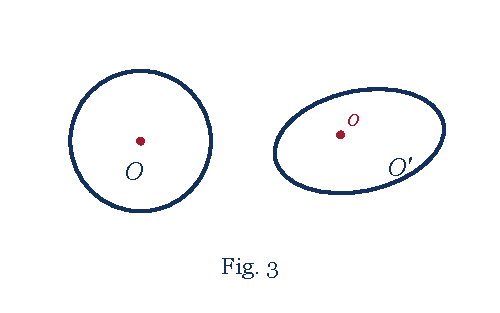
\includegraphics[width=0.6\textwidth]{figuras/pdf/cap01-fig3.pdf}
\caption{La esfera $O$, en su posición de equilibrio, se deforma en el
elipsoide $O'$; $o$ es el centro de gravedad desplazado.}
\label{fig:vol2-cap1-3}
\end{figure}

\section{Ondas planas}
\label{sec:vol2-cap1-ondas-planas-2}

\noindent\textbf{10. Ondas planas.} — Tomemos el plano de la onda como plano $xy$.

$\xi,\eta,\zeta$ serán funciones de $z$ y de $t$ solamente. Si la
vibración es transversal, tendremos
\[
\zeta=0
\]
\[
\xi=f\left(z-t\sqrt{\tfrac{\mu}{\rho}}\right)+f_1\left(z+t\sqrt{\tfrac{\mu}{\rho}}\right)
\]
\[
\eta=\varphi\left(z-t\sqrt{\tfrac{\mu}{\rho}}\right)+\varphi_1\left(z+t\sqrt{\tfrac{\mu}{\rho}}\right).
\]
El primer término en cada una de estas expresiones representa una
perturbación que se propaga hacia los $z$ positivos. El segundo, una
perturbación que se propaga hacia los $z$ negativos. Supondremos que
existe una sola de estas perturbaciones, sin lo cual habría interferencia
y nuestros razonamientos ya no serían válidos.

Pondremos, pues,
\[
\xi=f\left(z-t\sqrt{\frac{\mu}{\rho}}\right),\qquad
\eta=\varphi\left(z-t\sqrt{\frac{\mu}{\rho}}\right),
\]
por consiguiente
\[
\frac{d\xi}{dz}=f'\qquad \frac{d\eta}{dz}=\varphi'
\]
\[
\frac{d\xi}{dt}=-f'\sqrt{\frac{\mu}{\rho}}=-\frac{d\xi}{dz}\sqrt{\frac{\mu}{\rho}}
\qquad
\frac{d\eta}{dt}=-\varphi'\sqrt{\frac{\mu}{\rho}}=-\frac{d\eta}{dz}\sqrt{\frac{\mu}{\rho}}.
\]

La intensidad definida por la energía cinética media es proporcional al
valor medio de
\[
\left(\frac{d\xi}{dt}\right)^2+\left(\frac{d\eta}{dt}\right)^2.
\]

Calculemos ahora la energía potencial $\mathrm{W}$, considerando la
energía localizada en un elemento de volumen $d\tau$ y refiriéndola a la
unidad de volumen:
\[
\mathrm{W}=\mu\left(\alpha_1^2+\alpha_2^2+\alpha_3^2+\frac{\beta_1^2}{2}
+\frac{\beta_2^2}{2}+\frac{\beta_3^2}{2}\right)+\lambda\frac{\theta^2}{2}.
\]
En el caso actual todas las derivadas tomadas respecto de $x$ y de $y$ son
nulas, además $\zeta=0$, así como todas sus derivadas. Por tanto,
\[
\alpha_1=\alpha_2=\alpha_3=0\qquad \theta=0\qquad \beta_3=0
\]
\[
\beta_1=\frac{d\eta}{dz}\qquad \beta_2=\frac{d\xi}{dz}
\]
\[
\mathrm{W}=\frac{\mu}{2}\left[\left(\frac{d\eta}{dz}\right)^2+\left(\frac{d\xi}{dz}\right)^2\right].
\]

Puesto que $d\eta/dt$ y $d\xi/dt$ son proporcionales a $d\eta/dz$ y
$d\xi/dz$, las intensidades dadas por las dos definiciones son, pues,
proporcionales entre sí.

\section{Otras formas de las ecuaciones del movimiento}

\noindent\textbf{11. Otras formas de las ecuaciones del movimiento.} —
Hemos encontrado, para representar el movimiento
del éter, las ecuaciones
\[
\rho\frac{d^2\xi}{dt^2}=\mu\Delta\xi+(\lambda+\mu)\frac{d\theta}{dx}.
\]

Para que las vibraciones longitudinales tengan una velocidad
constantemente nula, es necesario que
\[
\lambda+2\mu=0.
\]
Introduzcamos esta condición, y las ecuaciones se convierten en
\begin{equation}
\begin{gathered}
\rho\frac{d^2\xi}{dt^2}=\mu\left(\Delta\xi-\frac{d\theta}{dx}\right)\\[3pt]
\rho\frac{d^2\eta}{dt^2}=\mu\left(\Delta\eta-\frac{d\theta}{dy}\right)\\[3pt]
\rho\frac{d^2\zeta}{dt^2}=\mu\left(\Delta\zeta-\frac{d\theta}{dz}\right)
\end{gathered}
\tag{II}
\end{equation}
Si las vibraciones son transversales, tenemos, en el origen del tiempo,
\[
\theta=0\qquad \frac{d\theta}{dt}=0,
\]
y $\theta$ permanece nulo en una época cualquiera. En efecto,
diferenciemos las ecuaciones (II)\footnote{El original dice aquí
«les équations (2)»; se trata evidentemente de las ecuaciones~(II) que
acaban de escribirse.~(N.~del T.)} respecto de $x,y,z$ y sumemos; resulta
\[
\rho\frac{d^2\theta}{dt^2}=\mu(\Delta\theta-\Delta\theta)=0
\]
\[
\frac{d^2\theta}{dt^2}=0
\]
\[
\theta=\mathrm{A}+\mathrm{B}t.
\]
$\mathrm{A}$ y $\mathrm{B}$ son independientes del tiempo. Si, pues, para
$t=0$ tenemos
\[
\theta=0\qquad\text{y}\qquad \frac{d\theta}{dt}=0,
\]
$\theta$ es idénticamente nulo. Es ordinariamente lo que se supone, y las
ecuaciones del movimiento toman entonces la forma
\begin{equation}
\rho\frac{d^2\xi}{dt^2}=\mu\Delta\xi\qquad
\rho\frac{d^2\eta}{dt^2}=\mu\Delta\eta\qquad
\rho\frac{d^2\zeta}{dt^2}=\mu\Delta\zeta
\tag{III}
\end{equation}
Pongamos
\begin{equation}
\frac{1}{\mu}\frac{du}{dt}=\frac{d\zeta}{dy}-\frac{d\eta}{dz}.
\tag{IV}
\end{equation}
Esta relación no define $u$ más que salvo una constante; supondremos que
para $t=0$ se tiene
\[
\xi=\eta=0\qquad \frac{du}{dt}=0.
\]
Pondremos del mismo modo:\footnote{El original repite aquí la misma
etiqueta «(IV)» para este segundo par de ecuaciones, en vez de darles un
número nuevo: las tres relaciones que definen $u$, $v$ y $w$, deducidas
unas de otras por la permutación cíclica de $\xi,\eta,\zeta$, forman un
solo sistema~(IV), y así lo cita Poincaré al final del párrafo («la
primera de las ecuaciones~(IV)» es la que define~$u$). Conservamos su
numeración. Además, en la segunda de estas relaciones el original imprime
$d\zeta/dy$ en lugar de $d\xi/dy$; es una errata
evidente, como muestran la permutación cíclica y la expresión de
$d^2w/dy\,dt$ que se forma a continuación.~(N.~del T.)}
\begin{equation}
\begin{gathered}
\frac{1}{\mu}\frac{dv}{dt}=\frac{d\xi}{dz}-\frac{d\zeta}{dx}\\[3pt]
\frac{1}{\mu}\frac{dw}{dt}=\frac{d\eta}{dx}-\frac{d\xi}{dy}.
\end{gathered}
\tag{IV}
\end{equation}

Formemos la expresión
\[
\frac{d^2w}{dy\,dt}-\frac{d^2v}{dz\,dt}.
\]
\[
\frac{d^2w}{dy\,dt}=\mu\left(\frac{d^2\eta}{dx\,dy}-\frac{d^2\xi}{dy^2}\right)
\]
\[
-\frac{d^2v}{dz\,dt}=\mu\left(\frac{d^2\zeta}{dx\,dz}-\frac{d^2\xi}{dz^2}\right)
\]
\[
0=\mu\left(\frac{d^2\xi}{dx^2}-\frac{d^2\xi}{dx^2}\right).
\]
Sumemos miembro a miembro:
\[
\frac{d^2w}{dy\,dt}-\frac{d^2v}{dz\,dt}=\mu\left(\frac{d\theta}{dx}-\Delta\xi\right).
\]
Por consiguiente,
\[
\rho\frac{d^2\xi}{dt^2}=-\left(\frac{d^2w}{dy\,dt}-\frac{d^2v}{dz\,dt}\right).
\]
Integremos respecto de $t$:
\[
\rho\frac{d\xi}{dt}=-\left(\frac{dw}{dy}-\frac{dv}{dz}\right).
\]
Según la hipótesis que hemos hecho sobre las condiciones iniciales, la
constante de integración es nula.

Las ecuaciones del movimiento podrán, pues, ponerse bajo la forma
\begin{equation}
\begin{gathered}
\rho\frac{d\xi}{dt}=-\left(\frac{dw}{dy}-\frac{dv}{dz}\right)\\[3pt]
\rho\frac{d\eta}{dt}=-\left(\frac{du}{dz}-\frac{dw}{dx}\right)\\[3pt]
\rho\frac{d\zeta}{dt}=-\left(\frac{dv}{dx}-\frac{du}{dy}\right)
\end{gathered}
\tag{V}
\end{equation}

Bajo esta forma, se ve que no cambian cuando se permuta
\[
\xi,\eta,\zeta \text{ en } u,v,w;\qquad u,v,w \text{ en } -\xi,-\eta,-\zeta;
\qquad \rho \text{ en } \frac{1}{\mu}\text{ y } \mu \text{ en } \frac{1}{\rho}.
\]
Efectuemos, en efecto, esta permutación sobre la primera de las
ecuaciones, la que define $u$: resulta
\[
-\rho\frac{d\xi}{dt}=\frac{dw}{dy}-\frac{dv}{dz},
\]
y efectuándola sobre la primera de las ecuaciones (V),\footnote{El
original dice aquí «la première des équations (IV)»; es una errata por
(V): la primera de las ecuaciones~(IV) es justamente la que acaba de
transformarse, y es la primera de las~(V),
$\rho\,d\xi/dt=-(dw/dy-dv/dz)$, la que, con
$\xi\to u$, $v\to-\eta$, $w\to-\zeta$, $\rho\to 1/\mu$, da la relación
siguiente.~(N.~del T.)} obtendremos
\[
\frac{1}{\mu}\frac{du}{dt}=\frac{d\zeta}{dy}-\frac{d\eta}{dz}.
\]

Estas ecuaciones no dan más que una primera aproximación en los medios
transparentes ordinarios, a causa de los fenómenos de dispersión: presentan
una mayor exactitud en el vacío.

% % ============================================================
% Capítulo II (Volumen II) — Teoría electromagnética de la luz.
% Comparación con la teoría elástica
% Traducción de "Théorie mathématique de la lumière II" (1892)
% Original: §§12-20, páginas impresas 19-33
% ============================================================
\chapter{Teoría electromagnética de la luz. Comparación de esta teoría con
la teoría elástica}
\chaptermark{Teoría electromagnética de la luz}
\label{cap:vol2-electromagnetica}

\section{Notación y ecuaciones de Maxwell}

\noindent\textbf{12.} Emplearé en todo lo que sigue las notaciones de
Maxwell, que recuerdo sucintamente, remitiendo para más detalles a la
propia obra del sabio inglés y a mi tratado titulado \emph{Électricité et
Optique}.

Consideremos primero la \emph{fuerza magnética}, cuyas componentes designa
Maxwell por $\alpha,\beta,\gamma$. En seguida, la \emph{inducción
magnética}, cuyas componentes son $a,b,c$ (cf. \emph{Électricité et
Optique}, t.~I, pp.~110 y sig.).

Se tiene, si no hay fuerza coercitiva:
\[
a=\mu\alpha,\qquad b=\mu\beta,\qquad c=\mu\gamma,
\]
siendo $\mu$ el coeficiente de permeabilidad magnética del medio.

En el vacío $\mu=1$. En los cuerpos diamagnéticos, se tiene $\mu<1$, y en
los cuerpos magnéticos $\mu>1$. Pero en la mayoría de los cuerpos, salvo el
hierro, el níquel y el cobalto, $\mu$ es extremadamente próximo a $1$.

Las experiencias de Hertz parecen demostrar además que, en el caso de las
corrientes oscilantes con extrema rapidez, la inducción no tiene tiempo de
producirse y todo ocurre como si $\mu$ fuera igual a $1$. La teoría
electromagnética supone precisamente que los fenómenos luminosos se deben
a corrientes alternativas semejantes, de igual período que las vibraciones
del éter. Estos períodos son alrededor de $10^5$ veces más cortos que los
de las corrientes observadas por Hertz.

\noindent\textbf{13.} Maxwell admite que existen, no solo corrientes de
conducción como las que se propagan en los cuerpos buenos conductores,
sino también corrientes de desplazamiento que se producen en los
dieléctricos e incluso en el vacío.

La intensidad $i$ de la corriente puede considerarse como la velocidad de
la electricidad; $\int i\,dt$ representa el \emph{desplazamiento}. La
resistencia de un dieléctrico crece, según Maxwell, con el desplazamiento;
de ahí se sigue que las corrientes de desplazamiento no pueden ser sino
corrientes alternativas extremadamente rápidas.

Sean $u,v,w$ las componentes de la corriente total; $p,q,r$ las componentes
de la corriente de inducción; $df/dt,dg/dt,dh/dt$ las de la corriente de
desplazamiento. $f,g,h$ serán las componentes del desplazamiento eléctrico.

En general:
\begin{equation}
u=p+\frac{df}{dt}\qquad v=q+\frac{dg}{dt}\qquad w=r+\frac{dh}{dt}
\end{equation}

Pero en los dieléctricos, como no hay conducción: $p=q=r=0$, y
\begin{equation}
u=\frac{df}{dt}\qquad v=\frac{dg}{dt}\qquad w=\frac{dh}{dt}
\end{equation}

Las componentes de la corriente están ligadas a las componentes de la
fuerza magnética por las relaciones:\footnote{En la segunda de estas
relaciones el original imprime $4\pi u$; es una errata evidente por
$4\pi v$, como muestran la permutación cíclica y la segunda de las
ecuaciones~(7) del §14.~(N.~del T.)}
\begin{equation}
4\pi u=\frac{d\gamma}{dy}-\frac{d\beta}{dz}\qquad
4\pi v=\frac{d\alpha}{dz}-\frac{d\gamma}{dx}\qquad
4\pi w=\frac{d\beta}{dx}-\frac{d\alpha}{dy}
\end{equation}

La fuerza electromotriz que se ejerce en un punto cualquiera tiene por
componentes $\mathrm{X},\mathrm{Y},\mathrm{Z}$.
\begin{equation}
\mathrm{X}=-\frac{d\mathrm{F}}{dt}-\frac{d\varphi}{dx}\qquad
\mathrm{Y}=-\frac{d\mathrm{G}}{dt}-\frac{d\varphi}{dy}\qquad
\mathrm{Z}=-\frac{d\mathrm{H}}{dt}-\frac{d\varphi}{dz}
\end{equation}

$\varphi$ es el potencial electrostático. $\mathrm{F},\mathrm{G},\mathrm{H}$
son las componentes de lo que Maxwell llama \emph{potencial vector}.
$-d\mathrm{F}/dt,-d\mathrm{G}/dt,-d\mathrm{H}/dt$ son las componentes de la
fuerza debida a la inducción de todas las corrientes que existen en el
campo. Se define también a veces el potencial vector como sigue:
$\mathrm{F},\mathrm{G},\mathrm{H}$ son las componentes de la fuerza
electromotriz de inducción que produciría la supresión brusca de todas las
corrientes existentes en el campo.

Se admite, sin que ninguna experiencia seria lo haya verificado, la
relación:
\[
\frac{d\mathrm{F}}{dx}+\frac{d\mathrm{G}}{dy}+\frac{d\mathrm{H}}{dz}=0.
\]

Se demuestra además que:
\begin{equation}
a=\mu\alpha=\frac{d\mathrm{H}}{dy}-\frac{d\mathrm{G}}{dz}\qquad
b=\mu\beta=\frac{d\mathrm{F}}{dz}-\frac{d\mathrm{H}}{dx}\qquad
c=\mu\gamma=\frac{d\mathrm{G}}{dx}-\frac{d\mathrm{F}}{dy}
\end{equation}

En un conductor, las corrientes de conducción satisfacen las relaciones:
\[
p=\mathrm{C}\mathrm{X},\quad\text{etc.}
\]
Este coeficiente $\mathrm{C}$ es la conductibilidad del medio; estas
corrientes de conducción son, pues, proporcionales a la fuerza
electromotriz.

Para las corrientes de desplazamiento, se tiene:
\[
4\pi f=\mathrm{K}\mathrm{X}.
\]
$\mathrm{K}$ es el poder inductor específico del medio; la corriente de
desplazamiento es, pues, proporcional a $d\mathrm{X}/dt$; esto explica su
corta duración, pues se anula tan pronto como la fuerza electromotriz se
vuelve constante.

Diferenciemos la primera de las ecuaciones (5) respecto de $t$.
\[
\mu\frac{d\alpha}{dt}=\frac{d^2\mathrm{H}}{dy\,dt}-\frac{d^2\mathrm{G}}{dz\,dt};
\]
por otra parte:
\[
\frac{d^2\mathrm{H}}{dy\,dt}+\frac{d^2\varphi}{dy\,dz}=-\frac{d\mathrm{Z}}{dy}
\]
\[
-\frac{d^2\mathrm{G}}{dz\,dt}-\frac{d^2\varphi}{dy\,dz}=\frac{d\mathrm{Y}}{dz}.
\]

Sumemos estas tres ecuaciones miembro a miembro, resulta:
\begin{equation}
\mu\frac{d\alpha}{dt}=-\left(\frac{d\mathrm{Z}}{dy}-\frac{d\mathrm{Y}}{dz}\right)\qquad
\mu\frac{d\beta}{dt}=-\left(\frac{d\mathrm{X}}{dz}-\frac{d\mathrm{Z}}{dx}\right)\qquad
\mu\frac{d\gamma}{dt}=-\left(\frac{d\mathrm{Y}}{dx}-\frac{d\mathrm{X}}{dy}\right)
\end{equation}
siendo las dos últimas ecuaciones obtenidas por permutación.

\section{Ecuaciones de Hertz}

\noindent\textbf{14.} Es posible hallar todavía una forma de ecuaciones más
apropiada para la comparación que tenemos en vista.

Habíamos puesto:
\[
4\pi u=\frac{d\gamma}{dy}-\frac{d\beta}{dz}
\]
con:
\[
u=p+\frac{df}{dt}\qquad\text{y}\qquad 4\pi f=\mathrm{K}\mathrm{X}.
\]
Se deduce:
\begin{equation}
4\pi u=\mathrm{K}\frac{d\mathrm{X}}{dt}=\frac{d\gamma}{dy}-\frac{d\beta}{dz}\qquad
\mathrm{K}\frac{d\mathrm{Y}}{dt}=\frac{d\alpha}{dz}-\frac{d\gamma}{dx}\qquad
\mathrm{K}\frac{d\mathrm{Z}}{dt}=\frac{d\beta}{dx}-\frac{d\alpha}{dy}
\end{equation}

Esta forma fue empleada por Hertz. Tiene la ventaja de ser simétrica y de
no contener más que dos cantidades: la fuerza electromotriz
$(\mathrm{X},\mathrm{Y},\mathrm{Z})$ y la fuerza magnética
$(\alpha,\beta,\gamma)$.

Habíamos encontrado en la teoría elástica las ecuaciones:
\begin{equation}
\frac{1}{\mu}\frac{du}{dt}=\frac{d\zeta}{dy}-\frac{d\eta}{dz},\quad\text{etc.}
\tag{IV}
\end{equation}
\begin{equation}
\rho\frac{d\xi}{dt}=-\left(\frac{dw}{dy}-\frac{dv}{dz}\right),\quad\text{etc.}
\tag{V}
\end{equation}

La analogía de forma de los dos sistemas es evidente, solo que no hay que
compararlos directamente, porque la expresión de la energía no se
presenta bajo la misma forma. Así pues, para hacer esta comparación,
modificaremos las ecuaciones (IV) y (V) de la manera siguiente.

Pongamos:
\[
\xi'=\frac{d\xi}{dt},\;\ldots,\;\text{etc.}\qquad u'=\frac{du}{dt},\;\ldots,\;\text{etc.}
\]

Diferenciemos las ecuaciones (IV) respecto del tiempo; resulta:
\begin{equation}
\frac{1}{\mu}\frac{du'}{dt}=\frac{d\zeta'}{dy}-\frac{d\eta'}{dz}\qquad
\frac{1}{\mu}\frac{dv'}{dt}=\frac{d\xi'}{dz}-\frac{d\zeta'}{dx}\qquad
\frac{1}{\mu}\frac{dw'}{dt}=\frac{d\eta'}{dx}-\frac{d\xi'}{dy}
\tag{8}
\end{equation}

\section{Comparación de estas ecuaciones con las de la teoría elástica}

\noindent\textbf{15.} Estas ecuaciones pueden compararse con las de la
teoría electromagnética de dos maneras:

\emph{Primer modo de comparación.} — Se puede pasar del sistema
electromagnético al sistema elástico cambiando cada una de las cantidades
escritas en la colocada debajo:
\begin{center}
\begin{tabular}{ccccccc}
$\mathrm{K}$ & $\mathrm{X}$ & $\mathrm{Y}$ & $\mathrm{Z}$ & $\mu$ & $\alpha$ & $\beta\quad\gamma$\\
en & & & & & & \\
$\rho$ & $\xi'$ & $\eta'$ & $\zeta'$ & $1/\mu$ & $-u'$ & $-v'\quad -w'$.
\end{tabular}
\end{center}

\emph{Segundo modo de comparación.} — Hay que cambiar
$\mathrm{K},\mathrm{X},\mathrm{Y},\mathrm{Z},\mu,\alpha,\beta,\gamma$ en
$1/\mu,\,u',\,v',\,w',\,\rho,\,\xi',\,\eta',\,\zeta'$.

Se trata ahora de interpretar este resultado.

En la teoría electromagnética se nos lleva, veremos más adelante por qué
razones, a admitir que, en una oscilación luminosa o en una oscilación
hertziana, la fuerza eléctrica es perpendicular al plano de polarización,
mientras que la fuerza magnética es paralela a ese plano.

\noindent\textbf{16.} La teoría electromagnética está fundada en
experiencias bastante seguras para conservar su lugar; son las teorías
elásticas las que deben conciliarse con ella y no ser más que una
traducción suya.

Ahora bien, en el primer modo de comparación, la fuerza
$(\mathrm{X},\mathrm{Y},\mathrm{Z})$ perpendicular al plano de polarización
corresponde a la velocidad $(\xi',\eta',\zeta')$ de la molécula de éter;
la vibración sería en este caso perpendicular al plano de polarización. El
poder inductor $\mathrm{K}$ corresponde a la densidad $\rho$ del éter; esta
densidad sería variable de un cuerpo a otro como $\mathrm{K}$; habíamos
visto que estaba permitido considerar $\mu$ como constante e igual a $1$:
el coeficiente de elasticidad del éter sería constante.

\emph{Esta interpretación es la de Fresnel.}

\noindent\textbf{17.} En el segundo modo, $\xi',\eta',\zeta'$ corresponden
a $(\alpha,\beta,\gamma)$, es decir que la velocidad corresponde a la
fuerza magnética, que es paralela al plano de polarización: el
desplazamiento del éter sería, pues, también paralelo al plano de
polarización; $1/\mu$ corresponde a $\mathrm{K}$ y sería variable como
él; $\rho$ corresponde a $\mu$ y sería, pues, constante:\footnote{El
original dice «$1/\mu$ correspond à K et serait variable comme; lui $a$
correspond à $1/\mu$ et serait donc constant», frase desordenada por una
errata de composición: según el segundo modo de comparación (§15),
$\mathrm{K}$ se cambia en $1/\mu$ y la permeabilidad magnética $\mu$ en
$\rho$, de modo que debe leerse «comme lui; $\rho$ correspond à $\mu$»,
como exige además la conclusión que sigue (densidad del éter
constante).~(N.~del T.)} luego la densidad del éter sería constante, y su
elasticidad variable.

\emph{Esta interpretación es la de Neumann.}

\noindent\textbf{18.} Vamos a comparar en particular la expresión de la
energía dada por la teoría de Fresnel y la que da la teoría
electromagnética.

Según Fresnel, la energía se compone de la energía cinética,\footnote{Las
cantidades $\xi_1,\eta_1,\zeta_1$, que el original no define aquí, son las
componentes de la velocidad, designadas en el §14 por
$\xi',\eta',\zeta'$.~(N.~del T.)}
\[
\int\frac{1}{2}(\xi_1^2+\eta_1^2+\zeta_1^2)\,d\tau,
\]
y de la energía potencial $\int\mathrm{W}\,d\tau$, poniendo:
\[
\mathrm{W}=\alpha_1^2+\alpha_2^2+\alpha_3^2+\frac{\beta_1^2}{2}
+\frac{\beta_2^2}{2}+\frac{\beta_3^2}{2}-\theta^2,
\]
aplicando al caso actual la fórmula dada en el §3 y
observando que:
\[
\mu=1\quad\text{y}\quad \lambda+2\mu=0,\;\text{o}\;\lambda=-2,
\]
puesto que se trata de ondas transversales.

La energía en la teoría de Fresnel tiene, pues, por expresión:
\[
\int\frac{\rho}{2}(\xi_1^2+\eta_1^2+\zeta_1^2)\,d\tau+\int\mathrm{W}\,d\tau.
\]

Para Maxwell se compone de la energía electrostática, más la energía
magnética, y tiene por expresión:
\[
\int\frac{\mathrm{K}}{8\pi}(\mathrm{X}^2+\mathrm{Y}^2+\mathrm{Z}^2)\,d\tau
+\int\frac{1}{8\pi}(\alpha^2+\beta^2+\gamma^2)\,d\tau.
\]

El primer término, la energía electrostática, es equivalente a la energía
cinética; en efecto, traduzcámoslo en notaciones de la teoría elástica: hay
que cambiar $\mathrm{K},\mathrm{X},\mathrm{Y},\mathrm{Z}$ en
$\rho,\xi',\eta',\zeta'$, lo que da
\[
\int\frac{\rho}{8\pi}(\xi'^2+\eta'^2+\zeta'^2),
\]
expresión idéntica a la de la energía cinética, salvo el factor numérico
$1/4\pi$. No hay que inquietarse por este factor, pues el sistema de
unidades no es el mismo en los dos casos.

La energía magnética es, por su parte, igual a la energía potencial. En
efecto, hagamos también la traducción.
\[
\alpha=-u'=-\frac{du}{dt}=-\frac{1}{\mu}\frac{du}{dt}
=-\left(\frac{d\zeta}{dy}-\frac{d\eta}{dz}\right),
\]
puesto que hemos tomado $\mu=1$.

Pongamos:
\[
\mathrm{V}=\alpha^2+\beta^2+\gamma^2
=\left(\frac{d\zeta}{dy}-\frac{d\eta}{dz}\right)^2
+\left(\frac{d\xi}{dz}-\frac{d\zeta}{dx}\right)^2
+\left(\frac{d\eta}{dx}-\frac{d\xi}{dy}\right)^2.
\]

La energía magnética será
\[
\int\frac{\mathrm{V}\,d\tau}{8\pi}.
\]

Pongamos todavía:
\[
\mathrm{U}=\left(\frac{d\xi}{dx}\frac{d\eta}{dy}-\frac{d\xi}{dy}\frac{d\eta}{dx}\right)
+\left(\frac{d\xi}{dx}\frac{d\zeta}{dz}-\frac{d\xi}{dz}\frac{d\zeta}{dx}\right)
+\left(\frac{d\eta}{dy}\frac{d\zeta}{dz}-\frac{d\eta}{dz}\frac{d\zeta}{dy}\right).
\]

Es fácil verificar la identidad:
\[
\mathrm{W}=\frac{\mathrm{V}}{2}-2\mathrm{U},
\]
o
\[
\int\mathrm{W}\,d\tau=\int\frac{\mathrm{V}\,d\tau}{2}-2\int\mathrm{U}\,d\tau.
\]

Digo que $\int\mathrm{U}\,d\tau=0$.

Para demostrarlo, basta demostrar que una de las tres integrales
\[
\int\left(\frac{d\xi}{dx}\frac{d\eta}{dy}-\frac{d\xi}{dy}\frac{d\eta}{dx}\right)d\tau,
\]
por ejemplo, es nula. La demostración se aplicará a las otras, que se
deducen de ella por simetría.

Esta integral se escribe también:
\[
\iiint\left(\frac{d\xi}{dx}\frac{d\eta}{dy}-\frac{d\xi}{dy}\frac{d\eta}{dx}\right)dx\,dy\,dz,
\]
estando las tres sumaciones extendidas a todo el espacio, o por
consiguiente
\[
\int_{-\infty}^{+\infty}dz\iint\left(\frac{d\xi}{dx}\frac{d\eta}{dy}
-\frac{d\xi}{dy}\frac{d\eta}{dx}\right)dx\,dy.
\]

La integral doble es nula, si suponemos que $\xi,\eta,\zeta$ se anulan en
el infinito; en esta integración, se supone que $z$ permanece constante,
dicho de otro modo se integra para todos los elementos de superficie,
contenidos en un plano $z=\text{cte.}$

Consideremos $\xi,\eta,\zeta$ como las coordenadas de un punto del
espacio: son funciones de $x$ y de $y$; a cada punto del plano
$z=\text{cte.}$ corresponde un punto del espacio; a todo el plano
corresponderá una cierta superficie cerrada; en efecto, para los puntos a
distancia finita, $\xi,\eta,\zeta$ son finitos; si el punto se aleja
indefinidamente en el plano en una dirección determinada, $\xi,\eta,\zeta$
tienden a $0$, puesto que se anulan en el infinito; la curva que
corresponde a esa dirección es, pues, cerrada. Como esta dirección es
cualquiera, se concluye que la superficie es también cerrada.

La integral estudiada representa la proyección de la superficie sobre el
plano de las $\xi\eta$.\footnote{El original imprime «plan des
$\zeta\eta$»; es una errata evidente por $\xi\eta$, pues el integrando es
el determinante funcional de $\xi$ y $\eta$ respecto de $x$ e $y$, y
$\zeta$ no figura en él.~(N.~del T.)} Como la superficie es cerrada, esta
integral es nula.

Queda, pues, solamente
\[
\int\mathrm{W}\,d\tau=\int\frac{\mathrm{V}\,d\tau}{2},
\]
y la energía magnética es equivalente a la energía potencial, salvo el
factor constante $4\pi$, que es el mismo que para la energía
electrostática.

Por consiguiente, hay buen acuerdo entre la teoría de Fresnel y la de
Maxwell.

La comparación entre la teoría de Neumann y la de Maxwell presentaría más
dificultades.

\section{Propagación de las ondas planas}

\noindent\textbf{19. Propagación de las ondas planas.} — Consideremos una
onda que se propaga hacia los $z$ positivos, siendo el desplazamiento
paralelo a $\mathrm{O}x$ (onda transversal): en este caso:
\[
g=h=0,\qquad f=\mathrm{F}(z-\mathrm{V}t),
\]
siendo $\mathrm{V}$ la velocidad de la luz.

Supondremos que $\mathrm{F}(z)$ es nulo para $z=z_0$, y para $z<z_0$, y
también para $z=z_1$,\footnote{El original imprime aquí $z=z^1$; es una
errata evidente por $z=z_1$.~(N.~del T.)} y $z>z_1$.

$\mathrm{F}(z)$ será distinto de $0$ solamente para $z_0<z<z_1$.

En estas condiciones, la perturbación estará circunscrita a una región
limitada por dos planos perpendiculares al eje de las $z$,
\[
z=z_0+\mathrm{V}t\qquad z=z_1+\mathrm{V}t.
\]

Estos dos planos avanzan simultáneamente, y su distancia permanece
constantemente igual a $z_1-z_0$. Entre ellos, y solamente ahí, el éter
está perturbado; fuera de ellos, todas las fuerzas son nulas.

Demos cuenta de este último punto.

Entre los dos planos tenemos corrientes paralelas al eje de las $x$ y que
tienen por intensidad total:
\[
u=\frac{df}{dt}=-\mathrm{V}\mathrm{F}'(z-\mathrm{V}t),
\]
puesto que $v=w=0$.

Para calcular la acción magnética de estas corrientes, vamos a aplicar la
ley de Biot y Savart. Según esta ley, una corriente rectilínea indefinida
ejerce sobre un polo magnético $\mathrm{M}$ una fuerza perpendicular al
plano que pasa por el polo y por la corriente, e inversamente proporcional
a la distancia del punto $\mathrm{M}$ a esa corriente.

Supongamos que la corriente se propaga en un hilo cilíndrico paralelo a
$\mathrm{O}x$, la acción magnética de este hilo sobre el polo $\mathrm{M}$
será igual en magnitud a la atracción que ejercería sobre ese polo una
materia atrayente repartida en el cilindro con una densidad igual a la de
la corriente; pero, para obtener su dirección, hay que girar esta última
fuerza $90^{\circ}$ alrededor de $\mathrm{O}x$.

\begin{figure}[ht]
\centering
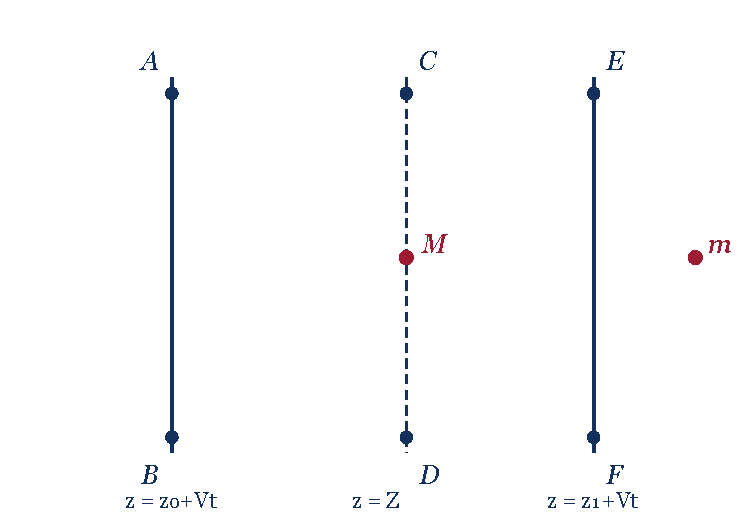
\includegraphics[width=0.7\textwidth]{figuras/pdf/cap02-fig1.pdf}
\caption{Los dos planos $z=z_0+\mathrm{V}t$ y $z=z_1+\mathrm{V}t$, con el
punto $\mathrm{M}$ interior y el punto $m$ exterior a la región
perturbada.}
\label{fig:vol2-cap2-1}
\end{figure}

\noindent\textbf{20.} Esta regla es todavía aplicable a una serie de
corrientes paralelas a $\mathrm{O}x$, como en el caso que nos ocupa.

Sea un punto $m$ exterior a los dos planos (figura~\ref{fig:vol2-cap2-1}):
consideremos una capa infinitamente delgada comprendida entre dos planos
$z$, y $z+dz$; podemos considerar la densidad $u$ de la corriente o de la
materia atrayente como constante en esta capa; y la atracción de esta
capa será la misma que la de un plano indefinido recubierto de materia
atrayente con una densidad superficial $\delta=u\,dz$. Se sabe que esta
atracción sobre un punto $m$ es constante e independiente de la distancia
de $m$ al plano y tiene por valor $2\pi\delta$.
\[
\delta=u\,dz=-\mathrm{V}\mathrm{F}'(z-\mathrm{V}t)\,dz.
\]

La atracción de toda la parte perturbada será:\footnote{El original
imprime $\mathrm{F}'(z-vt)$ en el integrando; es una errata evidente por
$\mathrm{F}'(z-\mathrm{V}t)$, pues $\mathrm{V}$ es la velocidad de la luz y
no hay ninguna otra velocidad en juego.~(N.~del T.)}
\[
\int_{z_0+\mathrm{V}t}^{z_1+\mathrm{V}t}-2\pi\mathrm{V}\mathrm{F}'(z-\mathrm{V}t)\,dz
=-2\pi\mathrm{V}\bigl[\mathrm{F}(z-\mathrm{V}t)\bigr]_{z_0+\mathrm{V}t}^{z_1+\mathrm{V}t}.
\]

Pero por hipótesis $\mathrm{F}(z_0)=\mathrm{F}(z_1)=0$: luego la atracción
buscada es nula.

No hay, pues, fuerza magnética fuera de los dos planos y, por
consiguiente, no hay inducción.

Sea ahora un punto interior $\mathrm{M}$ que tenga por ordenada
$\mathrm{Z}$. Tracemos el plano $z=\mathrm{Z}$, tendremos dos regiones por
distinguir: la primera, $ABCD$, a la izquierda de ese plano; la segunda,
$CDEF$, a la derecha. La atracción de la porción de la izquierda es igual
en valor absoluto a\footnote{El original imprime como límite superior de
esta integral una $z$ minúscula; es una errata evidente por la ordenada
$\mathrm{Z}$ del punto $\mathrm{M}$, como muestra el segundo miembro.~(N.~del
T.)}
\[
-2\pi\mathrm{V}\int_{z_0+\mathrm{V}t}^{\mathrm{Z}}\mathrm{F}'(z-\mathrm{V}t)\,dz
=-2\pi\mathrm{V}\mathrm{F}(\mathrm{Z}-\mathrm{V}t),
\]
puesto que $\mathrm{F}(z_0)=0$.

La atracción de la porción de la derecha tiene por valor absoluto
\[
-2\pi\mathrm{V}\int_{\mathrm{Z}}^{z_1+\mathrm{V}t}\mathrm{F}'(z-\mathrm{V}t)\,dz
=+2\pi\mathrm{V}\mathrm{F}(\mathrm{Z}-\mathrm{V}t),
\]
puesto que $\mathrm{F}(z_1)=0$.

Pero estas dos atracciones, estando dirigidas en sentidos contrarios, sus
valores absolutos deben restarse: lo que da para el valor de la atracción
resultante:
\[
-4\pi\mathrm{V}\mathrm{F}(\mathrm{Z}-\mathrm{V}t).
\]

La fuerza magnética entre nuestros dos planos no es, pues, nula.

% \input{03-integracion-ondas-planas/capitulo}
% \input{04-estudio-interferencias/capitulo}
% \input{05-teoria-reflexion-vitrea/capitulo}
% \input{06-propagacion-rectilinea/capitulo}
% \input{07-principio-huygens/capitulo}
% \input{08-hipotesis-kirchhoff/capitulo}
% \input{09-difraccion-ondas-convergentes/capitulo}
% \input{10-dispersion-helmholtz/capitulo}
% \input{11-dispersion-absorcion-anisotropos/capitulo}
% \input{12-polarizacion-rotatoria-mallard/capitulo}

\end{document}
